
%%%%%%%%%%%%%%%%%%%%%%% file typeinst.tex %%%%%%%%%%%%%%%%%%%%%%%%%
%
% This is the LaTeX source for the instructions to authors using
% the LaTeX document class 'llncs.cls' for contributions to
% the Lecture Notes in Computer Sciences series.
% http://www.springer.com/lncs       Springer Heidelberg 2006/05/04
%
% It may be used as a template for your own input - copy it
% to a new file with a new name and use it as the basis
% for your article.
%
% NB: the document class 'llncs' has its own and detailed documentation, see
% ftp://ftp.springer.de/data/pubftp/pub/tex/latex/llncs/latex2e/llncsdoc.pdf
%
%%%%%%%%%%%%%%%%%%%%%%%%%%%%%%%%%%%%%%%%%%%%%%%%%%%%%%%%%%%%%%%%%%%


\documentclass[runningheads,a4paper]{llncs}

\usepackage{amssymb}
\usepackage{todonotes}
\setcounter{tocdepth}{3}
\usepackage{graphicx}
\usepackage{enumitem}
\usepackage{url}
%\urldef{\mailsa}\path|{alfred.hofmann, ursula.barth, ingrid.haas, frank.holzwarth,|
%\urldef{\mailsb}\path|anna.kramer, leonie.kunz, christine.reiss, nicole.sator,|
%\urldef{\mailsc}\path|erika.siebert-cole, peter.strasser, lncs}@springer.com|    
\newcommand{\keywords}[1]{\par\addvspace\baselineskip
\noindent\keywordname\enspace\ignorespaces#1}

\begin{document}

\mainmatter  % start of an individual contribution

% first the title is needed
\title{Open Source Community \\ Joining \& Management}

% a short form should be given in case it is too long for the running head
\titlerunning{Open Collaboration and Peer-Production}
%\thanks{Please note that the LNCS Editorial assumes that all authors have used
%the western naming convention, with given names preceding surnames. This determines
%the structure of the names in the running heads and the author index.}


% the name(s) of the author(s) follow(s) next
%
% NB: Chinese authors should write their first names(s) in front of
% their surnames. This ensures that the names appear correctly in
% the running heads and the author index.
%
\author{UC Berkeley iSchool i290m class\footnote{The open collaboration \& peer-production (i290m) is a class on hands-on exploration of the theory and practice of open online collaboration. This report was collectively written by all students as a part of their class evaluation. Contributors are (by alphabetical order) : Agrawal, S., Benthall, S., Bora, R., Chen, T. K., Chuang, J., Hartnell, J.T., Jacksier-Chasen, F.W., Jervis, L., Maillart, T., Matta, P.,  Mcconachie, A.S., Merrill, N.J., Milutinovic, M., Nellimarkka, M., 
Nguyen, P.T., Ochigame, R.K., Perry, R.E., Petrozzo, C.A., Pham, C.P.C.
Puthyapurayil, S., Quast, T., Renold, A.,  Sedenberg, E.M.,Swigart, A.G., Tian,S., Trichur,V.V., Zhang, M.}}


\authorrunning{UC Berkeley iSchool i290m class}
%% (feature abused for this document to repeat the title also on left hand pages)
%
%% the affiliations are given next; don't give your e-mail address
%% unless you accept that it will be published
\institute{School of Information,\\
UC Berkeley, Berkeley}
%%\mailsa\\
%%\mailsb\\
%%\mailsc\\
%%\url{http://www.springer.com/lncs}
%\and Chair of Entrepreneurial Risks,\\ ETH Zurich, Switzerland}
%
%%
% NB: a more complex sample for affiliations and the mapping to the
% corresponding authors can be found in the file "llncs.dem"
% (search for the string "\mainmatter" where a contribution starts).
% "llncs.dem" accompanies the document class "llncs.cls".
%

%\toctitle{Lecture Notes in Computer Science}
\tocauthor{Authors' Instructions}
\maketitle

\newcommand{\mysubsubsection}[1]{\subsubsection{#1}\mbox{}\\}

\begin{abstract}

Here is the abstract

\keywords{open collaboration, peer-production, community joining, governance, education}
\end{abstract}
\clearpage
\section{Introduction}

Open collaboration and peer production systems comprise a significant
part of the Internet's infrastructure and content.
Practicioners within these systems recognize the importance of
\emph{community}\footnote{Fogel, K., Producing Open Source Software, \url{http://producingoss.com/en/technical-infrastructure.html}} in developing and sustaining these resources.
Paradigmatically, an open source software project is created and maintained by an on-line community.
The community engages in productive dialog using communication tools and contributes to
a common pool \cite{ostrom1990}, in a process that is sometimes called ``private-collective innovation'' \cite{vonhippel2003oss}.
It has been suggested that the core features of such collaborative
communities extend to other communities of practice, such as those
surrounding wikis, open data, and citizen science, as well \todo{by whom?}.

Our work is a contribution to the understanding of  open collaborative
communities and the underlying peer-production labor organization \cite{benkler2002} \todo{don't now what this reference tries to say}.
A critical aspect is the joining and management of these communities. There exists previous efforts in these domains, which have studied joining into these communities and impacts of the joining \cite{vonKrogh2003,Baldwin2006} \todo{more refs would be nice}.
We also focus on the joining process and on how
it integrates in the broader issue of community management.
We contribute by exploring this issue from a novice aspect and by examining non-coding communities, such as citizen science. The former aspect is important, as novel recent developers have different kind of problems than those experienced by the developers \cite{Begel2008}. The latter represent an emerging form of open collaboration, and worth of studies as such.

Our context for this study is a semester long course at UC Berkeley's School of Information, entitled ``Open Collaboration and Peer Production'' (i290m). The course itself applied many open source principles, for example
the students and instructors wrote this report in collaboration.
The students have spent the semester participating in an open
collaborative community of their choosing and reporting
their observations.
We have collaboratively developed a survey about our experiences joining
these projects, and the projects' organization and demographics. The total number of responders is 24, who are also taking part in the report writing.
By administering this survey to ourselves, we have collected data
that samples across a wide range of communities and researcher experiences.

\mysubsubsection{Discovering a Group to Join}
One of the central objectives of this report is to investigate factors that bring projects and potential contributors together. Prior to successfully joining and contributing to a project, newcomers must become aware of projects that are active and open to (or actively seeking) help, with available opportunities that resonate with the potential contributor's motivation to be part of an open source project. In the survey discussed here, we posed and analyzed questions relating to project outreach, contributor incentives, and the quality of the joining experience in order to gain novel perspective on the relationships between these factors for newcomers to a range of project types.\todo{I would just remove whole section}

%This report has also been \emph{written} collaboratively.
%The 24 respondents to our survey are all also authors of this paper.
%We have attempted to organize ourselves according
%to the best practices of open collaborative communities as discussed in literature.

In Section 2 we elaborate on the context of how we have written this report, as an exploration of this novel method is one of our main research contributions.
Section 3 provides some background literature which we draw from in
our survey design and analysis.
Section 4 explains our research methods, including quantitative
reporting and survey design.
Section 5 presents the results of our empirical work.
We discuss implications of our work in Section 6, and conclude. 



\section{Background}
\label{background}
A decade ago, open source software has appeared as an original self-organized ``Bazaar" way of producing software by opposition to commonly known ``Cathedral" top-down management \cite{raymond1999}. Like many surprising new phenomena it has also attracted research in management \cite{vonkrogh2006pro}, economics \cite{tirole2002some}, entrepreneurial legal studies \cite{benkler2002},  quantitative sociology \cite{crowston2005social} and even in complex systems physics \cite{maillart2008,tessone2011}. Open source software development has been understood as a private-collective innovation model in which developers gain both from their own (private) contributions as well as the (collective) work done by others \cite{vonhippel2003oss}. Despite notorious arising successes (e.g. Linux, Apache, Mozilla) and early recognition that fast growing Internet threats could be tackled better with full-disclosure (i.e. open source code) approaches to find and fix security holes in software (by opposition to non-disclosure  proprietary source code) \cite{}, it remained unclear how open source could prevail on proprietary business models.  The (apparent) benevolent commitment of large communities of developers was the most striking questions \cite{}. It is probably still the most fundamental question \cite{benkler2011leviathan}. But since the open source model has developed far beyond software programming as open collaboration for natural language knowledge production (e.g. Wikipedia), for industrial designs (3d printing, cars) \cite{raasch2009,pearce2012}, we at least know that open collaboration works well and probably far beyond most initial expectations. 


\cite{kuk2006strategic}

As companies get attracted by  ``bazaar" open collaboration and \linebreak peer-production models for innovation \cite{} and even production \cite{hamel2011first}, research tends to shift interest towards creating and maintaining user communities \cite{vonHippel2001} in closer collaboration with business  \cite{bonaccorsi2004ais} or more recently even completely integrated solutions within company boundaries \cite{}. For instance, one important requirement for getting a job at Facebook and in an increasing amount of Silicon Valley companies is precisely to have some open source software development experience, not only because the quality  of the code produced by the candidate can be checked {\it ex-ante}, but also because it helps build a sense of community in the company. In this precise case not only the expertise but also the social norms are internalized ! indeed motivation and social practice in open source projects have been found to be strongly related \cite{robert2006,vonKrogh2012}.

Open collaboration projects are rarely a completely horizontal bazaar. Most projects, when they reach a critical mass of contributors eventually self-organize with more or less implicit norms and sometimes with very well documented governance rules. It appears the process of shaping institutions goes along with the project development \cite{O'Mahony2007}. And in turn, the governance structure plays a role in the community structure, in particular how people join, contribute and eventually step down the project \cite{}. It is critical for a project survival to onboard enough contributors to offset those who leave. Governance structures can have deep influence on this, positive or negative. For instance, Wikipedia suffers from onboarding problems due to an over rigid governance system, which cannot account for community renewal \cite{halfacker2013}.

The number of software and non-software open collaboration projects has literally exploded with countless projects on Wikis and other online collaboration platforms such as Github or Sourceforge. For various intrinsic and extrinsic motivations to participate , like hedonic pleasure, reputation seeking or even to build a publicly available portfolio of achievements \cite{hars2001} , open collaboration projects attract the attention of an growing number of potential contributors, making even pressing the issue of tensions between (i) the necessity for projects to engage new contributors to offset natural attrition of ``old" developers, (ii)  the governance of continuously  renewing and growing communities, and (iii) its consequences for the on-boarding process of newcomers.

Enriched by the authors' immersion in the open collaboration project joining process over one semester, this collective work reports on the challenges of joining and how open collaboration communities should better manage it. Yet it is not the main aim here to describe its underlying production process,  the present report is also a collective work, which has been an important challenge for all the authors.  


\section{Context}
The  UC Berkeley iSchool Open Collaboration and Peer-Production (i290m) was designed to make sure students feel a sense of achievement conforming as much as possible the spirit of open source, with its easiest and more difficult aspects. While ensuring students achieve individually and collectively the requirements for the class, the instructors have acted as much as they could as community managers letting the class self-organize and help solve conflicting issues.


%\subsubsection{Citizen Science Intro}

As scientific data has become more open and accessible, either because of Federal regulations or changes in research culture, new collaboration opportunities were created among research teams. The citizen science movement is an example of crowd-sourced data collection or data processing that allows volunteers to access and collaborate in order to facilitate large-scale discovery. Volunteers, or citizen scientists, collaborate on a project or platform and have a variety of expertise levels. Although forms of citizen science have been seen throughout history, recent permutations of crowdsourced science were illustrated in projects like SETI@home\footnote{http://setiathome.berkeley.edu/}, where volunteers could donate their personal computer's processing power to help analyze radio telescope data for signs of extraterrestrial life. 

Most citizen science projects are hosted through academic organizations like universities, or non-profits focused on a specific research or issue area. Citizen scientists volunteer their time and expertise to projects of interest to them, and are usually not compensated for their research, unlike an academic scientific team would be. Often the crowd-sourced, citizen science projects may only represent a small fraction of an otherwise larger research area. Depending upon the level of community or volunteer engagement, a web-portal is often hosted to facilitate the collection of observations or data processing.



\subsection{Education \& Open Collaboration}
\label{classmotivations}

The {\it Open Collaboration and Peer-Production class (i290m OCPP)} is designed to combine hands-on exploration of the theory and practice of open online collaboration with students engaging multi-disciplinary literature about collaboration, joining and contributing to an existing open collaboration project involving programming or not. It recognizes that joining and getting integrated in project communities can be difficult but also greatly rewarding, and has been designed to facilitate integration and at the same time acquire the right tools to understand and possibly monitor how communities works. The open collaboration approach is remote from usual academic teaching settings and requires adaptation \todo{put more emphasis on the required adaptation : peer-review, task self-selection etc}. The i290m OCPP class offers the opportunity to discover and smoothly transition to this world. It is aligned with similar requirements increasingly requested by the industry, but also by the emerging field of reproducible data science, which has {\it de facto} embraced the open source model. Ironically open source software development  was initially inspired by academic research\cite{bezroukov1999oss}.

Besides attending and actively interacting in class as well as participating to an open collaboration project  \cite{classweb2013}, students have to produce two main deliverables : (i) guided individual assignments as blog posts on their community immersion structure (see Section \ref{qualitative_reporting}) and (ii) a collective report for students must pretty much self-organize to find a topic, pool their various experiences, compile and analyze data, discuss results and conclude. 

The report is an open collaboration project itself with the class being the community. The i290m OCPP class is designed to let as many contribution options as possible following {\it task self-selection} as well as many {\it peer-review} opportunities following the peer-production principles \cite{benkler2002}. Following the intrinsic motivation component of open collaboration students choose the open collaboration project(s) they want to contribute to, the way to address assignments that are pretty open, and how to engage in the collective report. In the end the success of the report relies on how students can collectively reuse what they have learned during the class and with the accumulated field experience. 



\subsection{Open Collaboration in the Classroom}
\label{opencollaborationintheclassroom}

From preliminary work including personal engagement in an open collaboration project and individual assignments, one main goal of the class is to produce a relevant collective report with no {\it ex-ante} guidelines and with self-organization as the default more. Instructors act as ``benevolent dictators" only when required or if extensive discussion are likely the impede to finish the report on time. We report on the main (self-)organization steps for this report.

\begin{enumerate}
  \item Collective report topic brainstorming {\bf (self-organized)} : recall the date and what has triggered a change in the syllabus
  \item Decision to design a survey {\bf (instructors)} : by the instructors
  \item Survey design {\bf (self-organized)} : question design (one by student) + categories
  \item Survey answering {\bf (instructors)} : everyone had to take the survey within a precise time window (recall it)
  \item Survey analysis {\bf (instructors)} :  each of us was asked to perform an analysis of her own proposed question(s).
  \item Report Latex format {\bf (instructors)} : choice for Latex by the instructors
  \item Learning Latex {\bf (self-organized)} : no crash course for Latex was provided in class. Those most confident with compiling installed or used Latex on their own computer. Others just edited the text without compiling. Mistakes would be corrected by those who could compiled the Latex code. The compiled document was sent regularly as a pdf to the mailing list. Surprisingly, there were little mistakes that prevented from compilation. On the other hand, the report has little sophisticated figures and tables.
  \item Producing a first chunk {\bf (instructors)} : all students were required to produce and commit a short paragraph commenting on the results provided to their own survey question.  
  \item Group formation to handle parts of the report {\bf (self-organized)} : 
  \item Production by groups {\bf (self-organized)} : To handle more integrative concepts and coherence of larger sections, groups were formed on a {\it task selection} basis during a class lab. Groups then drafted their sections on various collaborative editing platforms (e.g. etherpad, Google Docs). Sections built on chunks were finally uploaded as Latex files on the class repository.
  \item Peer-review {\bf (self-organized)} : Each section was reviewed by one or multiple peers until the document converged 
  \item Editing harmonization {\bf (self-organized)} : To harmonize editing -- to the extent it was possible -- we have tried to implement a few rules (use ``we", present tense by default).
\end{enumerate}


%\begin{figure}[ht!]
%\centering
%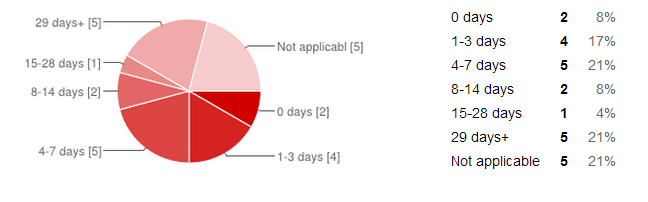
\includegraphics[width=90mm]{chapters/img/lurking_response.png}
%\caption{Network of survey topic organization and Progressive merging}
%\label{overflow}
%\end{figure}


\mysubsubsection{Other Patterns of Self-Organization}\\ 
We have found other patterns of self-organization in the class. To handle the large flows of commits for assignments, and commits to the report, committer rights were granted to volunteers, who reviewed and merged changes. Besides 
the official class website and github repository \cite{classweb2013}, we have used a variety of ad-hoc tools to help coordinate production and interactions. Etherpad, Google Docs, Google Forms are among these tools. A third pattern of self-organization is the way the instructors have tried to be less interventionist, precisely to allow (resp. force) more self-organization from the class. The effects of this policy are discussed later on in Section \ref{}.



\section{Methods}

\subsubsection{Survey Design Process}
To complement our qualitative understanding of the {\it joining process} we decided to design and run a survey. Each of us proposed a survey question and posted it on a Google Form \footnote{\url{https://docs.google.com/forms/d/1KnkSkM3f_QBRQeYfUXpyXspSqavjcClKS2DoWAz1fyE/viewform}}. We then categorized questions by assigning tags : communication, governance, contributions, social networks, joining (to be completed). One or more tags could be assigned to one question and has allowed to draw a bipartite network of relationships between questions (c.f. Figure, to be completed).

Once the first survey design was completed each of us took it. We debriefed the result in class and found several flaws that we described in a separate paragraph. However, the advantage of designing a survey in a collective way helped ensure that most questions would be relevant to most of us.

This is a starting point of course and in the future {\bf this survey could be iteratively improved}



\subsection{Qualitative Reporting}

The qualitative reporting is an integrative part of the class in the form of blog post assignments ($1000\pm500$ words per post). Assignments have covered the following topics by chronological order to allow for progressive mutual sharing of experience on the class website \cite{classweb2013}:

\begin{enumerate}
  \item {\bf First Contact with the Community} \\ 
This topic covers the motivations to choose a specific project as well as the process through which joining has occurred \cite{lakhani2005htu,robert2006,vonKrogh2012,}. Since the class organization (c.f. Section \ref{classmotivations}) set no constraints on which project could be chosen a broad variety of experiences where expected. Some reporting was expected on whether joining had been an informal process or a more formal established ``joining" script \cite{vonkrogh2003} and if this experience generalizes to all community joiners.\\

  \item {\bf Historical, Cultural and Demography Backgrounds} \\
Ideological, cultural and historical traits play a fundamental role in {\it sorting} communities. Evidence of this sorting has been brought regarding open source license types \cite{belenzon2009}. The evolution of an open source project and the condition under which it can be joined are path dependent. Deciding to join a project requires a good understanding of the cultural traits and social norms of the community. In this part, it was asked to report on the most relevant historical, cultural and demographic traits of joined projects and communities. \\


 \item{\bf Communication Infrastructure}\\
The success of open collaboration is deeply rooted in the capacity of community to organize with the help of online information systems (c.f. \cite{benkler2002} for theoretical argument), which in turn determine the way communities interact and keep records of the open collaboration innovation steps. \\

  \item {\bf Community Participation} \\
Blog post about community participation. Incorporate links to your project participation and engage the readings. Do they generalize to your experience? Or not? How? \\

  \item {\bf Governance \& Decision Process}\\
  One of toughest issue with large and rather horizontal communities is the decision process. The relevant question here is : How does a community make tough decisions? Open collaboration communities have shown some level creativity in that regard, with a large variety of governance models ranging from consensus ranging to benevolent dictatorship. The governance approach might be related to the project goals or simply be the result of path dependent history. Depending on the community, the governance structure can be informal or on the contrary clearly documented.

\end{enumerate}


\noindent Two blog posts (assignments) are due after the expected delivery of this report so their analysis cannot be included here :

\begin{enumerate}[resume]
\item {\bf Funding Sources :} Where does the funding for you community come from? Is there corporate sponsorship? A foundation that backs it? Do users donate? How does this affect the community's cooperative dynamics? Are there competing projects? How would you describe your project's role in the greater technical ecosystem?

\item{\bf Organization \& Project Modularity :} Does your project's community mirror the technical modularity of the project? How does it structure its collaboration--synchronously? Asynchronously? How does it get work done?

\end{enumerate}

\noindent The full assignment descriptions can be found on the class website \cite{classweb2013}.



\subsection{Survey Design}

\subsubsection{Survey Design Process}
To complement our qualitative understanding of the {\it joining process} we decided to design and run a survey. Each of us proposed a survey question and posted it on a Google Form \footnote{\url{https://docs.google.com/forms/d/1KnkSkM3f_QBRQeYfUXpyXspSqavjcClKS2DoWAz1fyE/viewform}}. We then categorized questions by assigning tags : communication, governance, contributions, social networks, joining (to be completed). One or more tags could be assigned to one question and has allowed to draw a bipartite network of relationships between questions (c.f. Figure, to be completed).

Once the first survey design was completed each of us took it. We debriefed the result in class and found several flaws that we described in a separate paragraph. However, the advantage of designing a survey in a collective way helped ensure that most questions would be relevant to most of us.

This is a starting point of course and in the future {\bf this survey could be iteratively improved}



\mysubsubsection{Survey Design}


To complement our qualitative understanding, we designed a survey {\it in collaboration} among class members. Overall, the questions reflected the course  readings and the participants' experiences within their respective open source communities. 

First, class participants generated questions in a lab session, with several participants incorporating additional questions remotely later on.  Then, the questions were categorized by concept tags: Communication, Demographics, Joining, Infrastructure, Motivation, Governance, Contribution, Finance, Social Network and Educational Experiences. From there, a effort was made to format the survey's  presentation and flow, informed by the categories, as well as reduce replications inquiries.

Questions used in the survey  are presented in Appendix \ref{app:survey_form}. As the survey was intended for class-use only, the class participants did not pilot it before collecting  responses. The final sample size was 24 responses, nn \% of the class \todo{TODO: FIXME}.

In the review of the question and during the analysis phase, we found several flaws described in a separate paragraph (see section \ref{link_to_limitations}\todo{fixme}). We believe these questions can and should be developed further; the current survey is a starting point and {\bf should be iteratively improved}. Some of the appropriate follow-up questions are included in this work. Furthermore, the collective design process ensured that most of questions were relevant to the majority, as can be seen in the following analysis part.
\subsection{Methods}
\label{sec:methods}

\mysubsubsection{Quantitative data}

As

\section{Results}








\subsection{Motivations for Joining \& Contributions}

 \mysubsubsection{The Difference between Experienced and Newcomers in Open Source}
To start my analysis, I divided the total number of responses into two categories based on how they answered the question : ``Prior to this project, did you have any experience in the past with open source projects?"
As a newcomer to open source communities myself, I wanted to analyze to {\bf see if there were any discernable differences or interesting trends between newcomers and ``veterans" of open source communities.} 
I started with the responses for how long did the individual lurk before making an attempt at reaching out to the community. We can see that in contrast to the ``No" group, the ``Yes" group has 2/11 or 18\% of people who didn't even lurk for a single day. On the  ``No" side, we can see that not  a single individual spent 0 days lurking and all of them had to spend at least 1-3 days lurking prior to joining.  This could indicate a stronger willingness to immediately dive in to a new Open Source community by the people who have had prior experience with them and a heightened shyness exhibited by the group with no experience with them before. The distribution for the YES  group is very disjoint when compared to the No group. For 71\%(5/7) of the Yes Group, it took them either more than a month or immediately to enter the OS community. This could indicate either {\it an extreme willingness or elongated hesitation that is not seen in the No Group} since there are no individuals that took 0 days and not as much of a frequency(20\% vs 43\%) of individuals that took more than 29+ days.  Statistically, {\it the distribution of the ``Yes" group is much more bimodal} with the peaks being at 0 days and 29+ days compared to the No group. 
 	Another interesting division between the two groups was their responses for the question ``what do  I plan on getting out of this contribution" For the Yes Group, the majority of them wanted not only experience in OS software but some sort of other reward like academic publication, career advancement, etc. However, this is decidedly false for the No Group where the majority wanted only experience in OS software or even nothing at all. This could be from the fact that because the Yes Group has contributed to Open Source communities before, they would need an extra incentive to join a new community while the No Group is simply excited to be part of this endeavor that they have never been on before. I think with further data, we could see if the requirement or desire for external incentives would increase linearly with the number of OS communities one would participate in.

Lastly, I thought it would be interesting to test if the two different groups would have differences in the roles that they play within their respective open source communities. I found that the number of roles a particular user from the Yes Group is significantly more than the number of roles a user from the No Group would take. This is to be expected as it is the No Group's first time. Other than that difference, the No Group had less developers and less documenters than the Yes Group but the same number of UX/Designers, Testers, and Analysts as the Yes Group. 




\mysubsubsection{Exploring Alternative Projects to Join}
A significant portion (~40\%) of the class had a clear idea at the beginning of the semester which project they wanted to join, and did not consider alternative projects. The majority of the class, however, spent some time investigating other open-source projects before settling on their selected project. The alternatives were rejected for a variety of reasons. Some projects were seen as having enough contributors; others were seen as not open to outsiders; {\bf (add more reasons)}. Three students actively sought to join a project but were frustrated in their attempts, due to a lack of response from the community, or more generally a outside appearance of {\it closeness} of the community.\footnote{The three projects are Bitcoin, Chromium, and Mozilla Open Badges.}



\subsubsection{True Motivations for Open Source Contribution}
{\bold 42. What do you want to get in return for your contribution?} My reason for asking about contributor motivation is to figure out if people really want anything in return for volunteering their time. Time is money, and it would be naive to think that everyone is truly altruistic. Out of 24 responses, a {\italic staggering} 50% want more experience in open source communities. This should be taken with a grain of salt because respondents are class peers. However, 25% are looking for career advancement or “nothing at all”, while a few receive satisfaction, skills, societal benefit, and web development experience from contributing. It is apparent that career advancement is a major reason for open source collaboration. Strangely enough, an equal amount of people want nothing at all, and only 2 respondents wanted academic recognition. Our sample size is small and academically biased, so it will be interesting extrapolate from a larger and more diverse sample size.


\mysubsubsection{The Reasons for Project Choice}
Much has been written about motivations in open source software
contributions \cite{vonKrogh2012}. It is insightful to surgey what are the main reasons 
for people when choosing their venue for participation -- particularly among
our class population, which is made up of people with a strong interest in peer production. 
The overwhelming majority ($67\%$) of respondents ($n=24$) reported that the project goals -- i.e, the audience and functionality --  was the most important aspect. Technical matters ( including the state of the project and the
skills required ) and community norms trailed far behind, with 17\% and 14\%
respectively. One respondent chose {\bf Other}, commenting ``my own interests and skills I can get". Even this statement does not necessarily go against the fact her/his own interests where aligned with the audience and even more with skills expected to be acquired. The narrative elaborations reveal that motivations related to project goals are determined by alignment with personal values, with skill sets. Some interesting quotes from the blog posts illustrate further the spirit of joining a project :

\begin{quotation} 
``As a self-confessed idealist,  what really sold me about the {\it Hypothes.is} project was the their huge plans. I liked the big picture thinking."
\end{quotation}

\begin{quotation}
``A shared, peer-distributed datastore is its own reward."
\end{quotation}

\begin{quotation}
``I wasn't the most technically sound person so i knew that i wouldn't 
necessarily be contributing to the coding of the project. I wanted to be apart of a 
project that did good in the world because i believe the power of open source is 
underutilized in philanthropy."
\end{quotation}

\begin{quotation}
``To me, all open source projects have a benign motto. Therefore, my decision criteria mainly
 depended on the technical aspects of the project. I want to contribute in an area where I 
 can understand their system better and contribute to the best of my abilities."
 \end{quotation}

\begin{quotation}
``I am very interested in technology that facilitates spreading and creating knowledge, 
and have struggled first-hand with the current limitations in the process of consuming, 
sharing, and building upon scientific literature."
\end{quotation}

Of course, people elaborated on the other motivations as well:

\begin{quotation}
``Project seemed like a good technical challenge, from which I could improve my Javascript 
skills and general code organization."
\end{quotation}

\begin{quotation}
``I wanted a community that was open and friendly, and I found that to be more 
important than anything else."
\end{quotation}




\subsubsection{Timed Commitment} Seventy-one percent of survey respondents contributed 1 to 3 hours per week on average to their open source projects, while 17\%
committed 4 to 6 hours on average and 13\% 10+ hours on average. None of survey respondents selected 7 to 9 hours on average. This question warrants 
a qualitative investigation to further understand participants' reasons for committing a low, medium, or high interval of 
time to their projects. 


\subsubsection{\bf Roles in the Community} Fifty-nine percent of the survey respondents identified themselves as fulfilling more than one 
role within their communities. Of the 24 respondents, 41\% fulfilled one role; 30\% two roles; 21\% three roles; and 8\% for 4+ roles. 
The results illustrate collaborators not only wear different hats within the communities, but they possess additional skill sets suggesting the majority 
are willing to contribute across a variety of project tasks. Further study is needed to understand the reasons participants use multiple skill sets for their projects  

While a majority contributed more than one skill, most survey respondents identify as developers. Of the 24 survey responses, 25\% individuals function as Developers; 
18\% as User Experience Designers; 18\% as Documenters; 12\% as Testers; 10\% as Editors; 10\% as Other; and lastly, 8\% as Analysts. This suggests a majority of the participants contribute through software development 
within the community. Of the survey participants, the combined roles of Developer and User Experience Designer occurred most frequently.  
 
The participants who categorized themselves as Other warrants additional follow-up questions in hopes of understanding any unidentified niche roles 
trending within the open source and peer collaboration space. Further study into the similarities and differences of each role within different types of open source 
communities may illicit a more nuanced picture.




\subsection{Case Study: Experiences as a non-technical contributor on a technical open source project}
 
In the world of open source, attention is often focused on the coding aspect of the project and little focus is often given to the “non-technical” tasks that are required to keep a project smooth and accessible. On the particular project of MIFOS, an opensource micro-finance software, non-technical contributors are almost treated as second-tier contributors or afterthoughts. This can be seen simply by how non-technical contributors are received versus their technical counterparts. When one first navigates to their “How to contribute” page, the section greets you with a technology overview which guides one through the process of code submissions, coding standards, and commit privileges. There is no mention on the page of any alternative methods that one could contribute to the project. Only upon further digging and navigating through 2 more pages into the actual tasks list that are being requested can one find the non-technical tasks that are available for contributors.

While it is very understandable how software based projects would focus the majority of their attention on garnering focus toward coding based contributions, non-technical contributions should not be neglected. The very nature of open source is dependent on open adoption of their project. The foundation of OS was for the projects to be transparent and adoptable so that a community can easily grow around thrive around it. In the context of technical vs non-technical contributions, while technical contributions of coding adds to the core of what the project is, non-technical contributions help foster and grow the community to improve the front-end perceptions of the project as well as adoption accessibility. In a typical project, documentation and reporting is what helps newcomers acclimate to the new environment. Mailing lists help foster community and cohesion.

In most projects, contributors do not label themselves as technical or non-technical contributors. Technical contributors or coders also help documentation and contribute to mailing lists as well.  However, the infrastructure of the OS project may draw that line for them. In MIFOS, the code developers have their own mailing list. Suggestions from a non-code focused developer are submitted to the website instead of having them directly communicate over a forum.  

Developers are further divided into task teams which further segregate the community. While this division may prove to increase efficiency by virtue of modularity, it also alienates members of the community and creates more ignorance or negligence of what needs to be done overall. From the results of the survey, we can see that almost a majority of respondents listed lack of clear documentation or mailing list activity as their response to what problems they encountered. More attention needs to be drawn to the non-technical aspect of Open Source projects in order to increase front-end fluidity and community cohesion.

\subsection{Joining an Open Source Project}

\mysubsubsection{The joining process}
Based on reports from students who joined a host of different kinds of open source projects for the Fall 2013 semester, we can begin to get a glimpse of the onboarding process and the various forms it takes across projects. Some wrote an introductory email \cite{Pham-09-17} and were accepted, while others had to sign a contract \cite{McConachie-10-08}. The structure of the community seems to be important here. Several students point out that a clear infrastructure made it easier to join, since it guides through the joining process and explains how to contribute. Clear and thorough documentation was another factor, however some reported that missing documentation was the initial trigger for starting to contribute. In general, individuals joining open source projects experience a spectrum of responses from warm and welcoming to none at all. Often this depends on the {\it joining script} they use \cite{vonKrogh2013}. The following is a summary of the range of responses students received. 

Most first contacts that got through were very personal. While some responses were extremely helpful and welcoming, a number of projects didn't respond to first-contact attempts. Whether the non-responses were a result of potential participants attempting to join in the ``wrong'' way or through the wrong channel,  projects trying to attract new contributors would do well to make the path to contributing easy and clear. A number of students reported coming across neglected project documentation infrastructure, like unused mailing lists.  A related obstacle to entry for beginners is that convoluted infrastructure can be overwhelming for beginners. Even where projects have explanatory infrastructure for {\it newbies}, the proliferation of too many communication channels sometimes pushed potential contributors to find a human and reach out directly. In the words of the students, this is what the experience was like:

\begin{quotation}
``I scanned through the archive, which goes back to roughly 2011, and it doesn't seem to be heavily used. Many posts for help or feature requests are of poor quality and go unanswered while most bug reporters are pointed to Github issues. There isn't much development discussion occurring on the list.''\\�

``...the forums, the wiki, the mailing lists, and the issue tracker are all separate systems with their own login info.''\\

``...the publicly visible development channels are quiet. A foundation forum is accessible to founding members, but not to normal contributors. A wiki is open to developers, but little discussion takes place here, and shockingly few edit wars.''\\
\end{quotation}

Another factor that has been reported is the prior knowledge of the contributors \todo{do you mean personal/social connection ?}. Generally if contributors were known as interesting people it had a positive impact on the project.


\mysubsubsection{Lurking Behaviors and Initial Contact}\\
We explored lurking behavior and found that projects using Github as well as those using FAQ had longer lurking times. On the contrary, projects with formal onboarding material or {\it beginner bugs} identified had lower lurking time (see Table \ref{tab:lurking_time_regression}).

\begin{table}
\centering
\begin{tabular}{lccc}
Factor & $\beta$ & $\sigma(\beta)$ & significance \\
\hline 
Uses Github & 2.291 (1.170) & 0.480 & 0.071* \\ 
Has newcomer bugs & -0.309 (0.906) & -0.081 & 0.739 \\ 
Has a FAQ & 1.114 (0.834) & 0.290 & 0.203 \\ 
Has onboarding instructions & -1.372 (0.975) & -0.352 & 0.181 \\
\hline
Previous OCP experience & 0.104 (0.737) & 0.032 & 0.890 \\ 
\hline 
\end{tabular} 
\caption{Explaining lurking time. This model has rather good fitness (adj. $r^2$ 0.134); however other than the Github factor fail to achieve statistical significance. Without the beginner bug question, we can report significantly higher adj. $r^2$ in 0.185 without effects on other questions significance}
\label{tab:lurking_time_regression}
\end{table}

These results draw a mixed figure of the phenomena: having a FAQ might indicate complexity of the project or the level of institutionalization, which could explain our findings. However, the negative factor on {\it onboarding instructions} indicates that lurking might not be only about getting familiar with the community, rather also following and understanding the behaviors of the community, often explicated in on-boarding information.  We found it interesting that open collaboration project (OCP) development was clearly a non-significant factor and that the coefficient is approximately zero, therefore indicating that this control variable has no impact on lurking time.

Most participants answered that they {\bf have been lurking} prior to contacting the project, although the lurking period is widely spread\footnote{$21\%$ answered that the question is not applicable for them and their project.}.  


\begin{figure}[ht!]
\centering
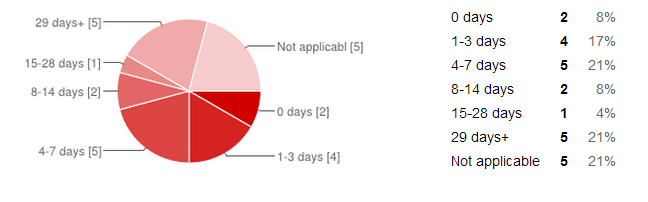
\includegraphics[width=120mm]{chapters/img/lurking_response.png}
\caption{Lurking Period}
\label{fig:lurking_period}
\end{figure}

About half of the people used private mail or through private email to get in contact with the community. While social networks might have an impact on open source software, social media was only used by one participant. This suggests that the impact of social media is still not well understood. In summary, personal email or to the mailing list remains the main initial communication means for joining.

\begin{figure}[ht!]
\centering
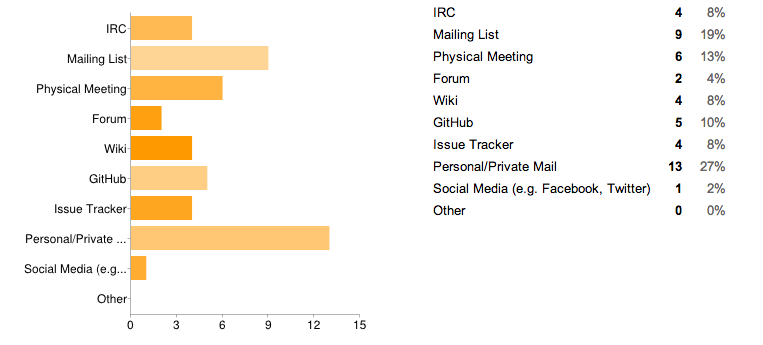
\includegraphics[width=120mm]{chapters/img/initial_contact.png}
\caption{Initial Contact}
\label{fig:initial_contact}
\end{figure}

\mysubsubsection{The Importance of Personal Touch}
We found personal contact to be an important factor in the process of finding a group to join. Forty-four percent of respondents reported that they first heard about the project they eventually joined through human contact, and 40\% cited a physical meeting or personal email exchange as the means taken to initially communicate with their project about the possibility of contribution. It is possible that this communication pattern may be biased by the unique academic setting that all respondents were in, as part of a course that facilitated in-person discussion about possible projects to join. Several respondents ended up participating in projects that other classmates were heavily involved in. Further research is needed to investigate whether most contributors to open collaboration projects have some personal connection with the project, or if the present results are unique to our specific situation.


\begin{figure}[ht!]
\centering
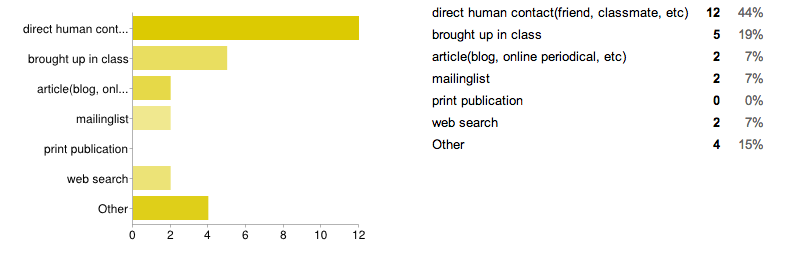
\includegraphics[width=120mm]{chapters/img/importance_of_personal_touch.png}
\caption{Importance of personal touch}
\label{overflow}
\end{figure}


Personal contact was also an important outreach method for 46\% of the projects surveyed, and we further examined whether this finding was related to the size of the group. An open-ended survey question about project outreach was qualitatively coded for personal contact, with responses which indicated efforts such as small in-person meetings and/or project member attendance and outreach at hackathons, workshops, conferences, and other community events that were not only held online. We did not find a dependence between group size and outreach through personal contact (Fisher’s Exact Test, p = 0.55). This finding suggests that both large and small groups rely on various types of in-person outreach to recruit new contributors. Since these organized group meetings are a common first contact point for many potential contributors, further research is needed to identify how different types and approaches to personal modes of outreach impact the recruitment of individuals with specific skills or motivations.


Most of the classmates report back that they have had physical contact to at least one of the projects contributors. This can have been through a talk at the university, through other classmates or through work. They report back that this was the initial trigger that made them know about the project by at the same time breaking down entry barriers since it was easier to get information when needed. Therefore many of the project are somehow connected to the Bay Area, which might be surprising as open source project often are seen as international where physical space plays a secondary role.

\mysubsubsection{Openness and Responsiveness}\\
Many respondents report that the community openness is an important criteria when joining. They actively searched for information about how to join and how other people joined. The more information that was available to more likely people wanted to join (See fig. \ref{fig:personal_touch}). Also responsiveness is reported by many as an important factor. Many wrote to the mailing list or tried to contact the community before committing work. The quality and quantity of the initial communication set the stage of how the community was perceived. It is not surprising that positive feedback was motivating people to contribute.

\mysubsubsection{First_contribution}
Most people describe that they were unsure about their first contribution. There were several concerns which made it hard to get it going. These were often related to the overall process and the quality of the committed information. Mostly the first commit was rather small and isolated. Several used the projects bugtracker to find some information on what to work on.

\mysubsubsection{Onboarding Problems}
$25\%$ of the people reported that lack of proper documentation is the biggest problem they faced while contributing to open source projects. This makes the joining process very time consuming, which trigger delays before the very first contribution can actually be done. When a project involves software development,  having an up and running installation to tinker with is an another important onboarding issue. Some respondents ($19\%$) contributing to technical open source projects reported that they had troubles with installing and running the software on their machines. In spite of the availability of the documentation, they could not find a solution to their problems. The responses to their mails are very cryptic and are mostly stuck with solving the problem on their own, resulting in wastage of time. Similar to this issue is the high complexity of the code base which required lot of time to even understand the project. Because of this it has been hard to get up to speed and make a contribution to a current need or issue in the project.

\begin{figure}[ht!]
\centering
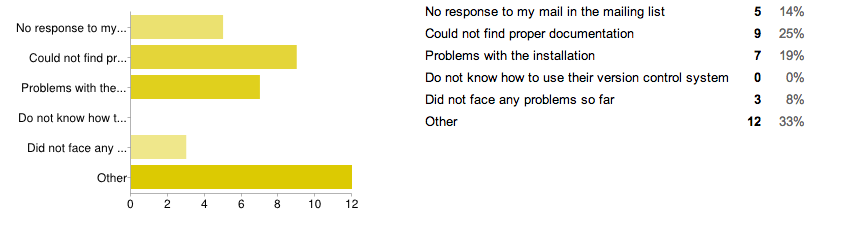
\includegraphics[width=130mm]{chapters/img/problems_faced.png}
\caption{Problems faced by new contributors. {\bf Can you say more about Other ?}}
\label{fig:problem_faced}
\end{figure}

Another major problem reported is the lack of sense of community in the open source projects respondents wanted to join (\todo{does it come from other in Figure \ref{fig:problem_faced}}). Some complained that they did not get any response or favorable warm response if at all, to their introduction mail in the mailing list. This led to a sense of alienation and fear of contribution by the newbies \todo{do we have any example of someone having left a project because of this?}. 

%% moved stuff to discussion -- Matti







\mysubsubsection{FAQs and Onboarding Documentation}
Around 50\% of projects have no actual FAQ or onboarding documentation, so there may exist opportunities to help newcomers by creating this type of content. Only 8\% have an initial contact designated. That may be due to varying organization structures, possibly even reflecting a deliberate choice to have the entry point be distributed and/or in flux (adaptive to varying needs). Both the contact people and the dispatch of inquiries may isimply be handled on ad hoc, informal, voluntary bases. Since members probably do have forum identities or other contact points, presumably, newbies can take initiative and contact them.

\begin{figure}[ht!]
\centering
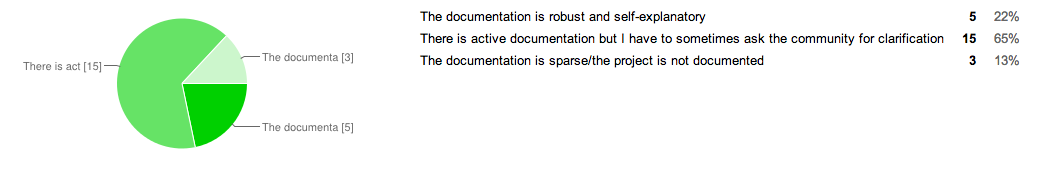
\includegraphics[width=120mm]{chapters/img/documentation.png}
\caption{How well are projects documented }
\label{overflow}
\end{figure}

Onboarding practice documentation may exhibit the potential for qualitative analysis, such as text analysis. (Perhaps just raising the issue  to project leads would raise interesting questions about governance and organizational processes). There might be correlations between FAQ/onboarding info available and the org structure/governance of the actual projects\todo{very interesting point !}. A summary follows of the projects and the types of onboarding guidance they provide, which often indicate the types of newcomer being targeted:

\begin{itemize}
\item {\bf Hypothesis:} Development-centric (may be sufficient for their needs)
\item {\bf Peerlibrary:} Several different ways to contribute are listed and described. Since a member of our own group wrote it, it may not be a coincidence that this is one of the best all-purpose joining guides.
\item {\bf Mozilla PDF:} Mentions that all ideas are open (also,is mainly bug, feature, and development-oriented)
\item {\bf Courtlistener:} Has a great "ways to help" page \todo{insert url as footnote plz}
\item {\bf Facebook React:} Developer and bug-centric, but also apologizes that they are still working on both improving transparency and creating a smoother, easier flow for contributors.
\item {\bf Chromium:} Developer-centric
\item {\bf Civi-CRM:} no FAQ, but does express and embrace a "just dive in" culture, which may be sufficient
\item {\bf Geonode:} The "about us" page is a bit FAQ-like, with some info on getting started, contact info, etc.
\item {\bf OaklandWiki (a site of the Localwiki project):} the product is a wiki which requires no login to contribute content. One can immediatley add or edit content with no account. There is no apparent moderation, so they may someday have problems with quality or spam.
\item {\bf Mifos: } Complex options, but anyone can create an account. The ways to contribute are mainly technical, and some contribution screens require login, but many volunteering opportunities and tasks can be found in their volunteer sections-- the site was a bit fragmented. Some confusion may arise from the availability of both "contributor" and "volunteer" sections and subsections. The technical and non-technical areas had various options and areas. Presumably more options to participate become available after creating a free account for login access.
\end{itemize}

The other projects do not yet have any FAQ or onboarding documentation. Since there may be shared responsibility, or unclear responsibility, for marketing and community-building in these projects (these functions may be absorbed by members in decentralized fashion), it is sometimes not clear whether improving onboarding information would benefit the projects, or decisions have already been made that the current practices are sufficient. There was a striking variety of information that was available to help people with various backgrounds and skill levels join the communities. 










\subsection{Community Demographics \& Project History}



{\bf Question about Project Founding Date}
We asked the question about project founding date to consider relative ages of different FLOSS communities. This set of ages reported helps to identify different stages of FLOSS project development. We expected that there might be patterns in communities as they are born, grow, reach maturation, and persist over time, or fizzle out. 

Among the projects surveyed, all started after 2001, and nearly half sprang up during or after 2011. As small a range as this is, we can consider the projects according to four ages: new (born in or after 2011), settling down (between 2008-2010), established (between 2007-2005), and anything older old. (If surveying a larger community, the ranges might be collapsed differently to account a more uniform spread across a larger range of years.)

{\bf Diversity Questions}
This set of questions aims to gather information on various kinds of diversity within projects. As has been cited in various surveys with respect to gender diversity, FLOSS projects suffer from a dearth of women contributors. \footnote{See a number of sources on women in FLOSS communities here: \url{http://geekfeminism.wikia.com/wiki/Open_Source_Software}} We expect to see similar patterns in other demographic groups that tend to be underrepresented elsewhere in society.

Metrics related to diversity are challenging to define, and answers will reflect biases of answerers about definitions of diversity and participation (with whom) in the project and community. Nonetheless, we expect responses to shade in our understanding about the demographics of different projects, and hopefully correlate with other community characteristics. Ultimately, we are curious about the relationship between diversity and how participation plays out. The additional question will hopefully capture more broad statements and intuitions about diversity (and perhaps other types of diversity) in the community.

According to respondents, project communities are made up of people of diverse backgrounds and experiences on all levels except the socioeconomic level. What we can gather from the write-in answers, however, is that respondents experienced some difficulty in assessing the demographics of all the communities due to remote communication and lack of demographic data collection. 

Still, comments from those who were able to report on demographics suggest a trend that FLOSS project leadership and contributors are mostly middle- to upperclass males who are mostly from developed countries. 

These questions on diversity and their responses necessitate deeper study in the future to better understand the demographic make-up across a wider range of FLOSS communities and how such diversity affects communication, movement, innovation in projects. 




\subsection{Communication \& Tools}

\subsubsection{Personal Connections}

To understand whether open source collaborators actually try to know each other on a personal level, we asked them if they knew any of the collaborators to the project personally. Out of the 23 responses, 12 said that they knew other collaborators personally. Furthermore, we asked the people who knew other collaborators if they ever discussed their contributions with the others. 10 out of 12 people replied in the affirmative. 

{\it A good followup question would have been if this personal connection helped them in any way with their contribution, but it was too late to add it}



\mysubsubsection{Regular Community Meetings}
{\it Are regular community meetings related in some way to project governance and the ease or difficulty of a joining script?}

Looking into the data from our survey and experience as a class. It seems that regularly held meetings, do help with good project governance. In our experience from class, it seems that regular meetings play a significant role in driving project progress. This may be a result of the general environment, that the course demographic is specifically busy graduate students. In the survey results, it will be interesting to see if respondents who claimed their community holds regular meetings, found the project governance and the joining script to be easier, simpler, or more user friendly. From my own experience with the IPython community, regularly scheduled meetings, whether in person or remote, seemed to be an important tool for decision making for medium and long term project goals. For example, the community holds a meeting along with each release, presently every six months, for core developers. The main purpose of the meeting is to create a roadmap for the next release, a seemly important step for making progress in the project.


\subsection{Organization and Governance}

\mysubsubsection{Regular Community Meetings}
{\it Are regular community meetings related in some way to project governance and the ease or difficulty of a joining script?}

Looking into the data from our survey and experience as a class. It seems that regularly held meetings, do help with good project governance. In our experience from class, it seems that regular meetings play a significant role in driving project progress. This may be a result of the general environment, that the course demographic is specifically busy graduate students. In the survey results, it will be interesting to see if respondents who claimed their community holds regular meetings, found the project governance and the joining script to be easier, simpler, or more user friendly. From my own experience with the IPython community, regularly scheduled meetings, whether in person or remote, seemed to be an important tool for decision making for medium and long term project goals. For example, the community holds a meeting along with each release, presently every six months, for core developers. The main purpose of the meeting is to create a roadmap for the next release, a seemly important step for making progress in the project.


\subsubsection{Visibility of Work in Open Organizations}

In an open source project, whether software or non-software, infrastructure has made it possible for contributions to be visible the community in some way. Software projects are supported by version control and issue or bug tracking and non-software projects such as a wiki are supported by wiki technology which essentially provides version control for documents. Both types of projects are also often supported by additional infrastructure such as IRC chats, mailing lists, discussion forums and blogs. An important affordance of the infrastructure supporting the work units of a project is that the infrastructure typically makes work units visible to other community members. Examining one infrastructure technology which supports a wide range of open source projects, GitHub, reveals a significant number of features that attach ownership of work units to project participants. GitHub's Issues feature, where the issues themselves can be considered a unit of work, allows one of more contributor to be assigned to an Issue. Similarly a Pull Request on GitHub is attributed to the author and the author remains visible in the code through Git's 'blame' feature, where lines of code can be annotated by contributor. Looking at a wiki such as Wikipedia, the units of work are the actual contents of each wiki and are therefore always visible. Wiki technology also allows for changes made to a page to be attributed to a specific author. While it is not a revelation that open source projects make visible the work of community members, it is worth examining the benefits to the organization and distribution of work tasks, and the community structure that arises out of openness.

{\it Ownership} - One important effect of visible work in open source projects is the ownership of work before and after completion. Before a task is completed, it is highly useful for the task to be assigned to or claimed by a community contributor. First, the visibility of ownership of a work unit, prevents other community participants from unnecessarily duplicating efforts to complete the task. Reflecting on participating in authoring parts of this paper, little writing was completed before contributors were assigned to work on specific sections of the paper. When contributors know which section or subsection they would author, there was some organizing of subgroups and then further delegation of tasks to subgroup members (At least for this section). Section the visibility of ownership of work motivates many contributor to participate. For example, a GitHub user name is now a common feature on a software developers resume or requested by a potential employer. This suggests that participation in an open source project could lead toward a future gain of some sort of status for a potential employer.

{\it Coordination and Delegation} - The next important effect of visible work in open source projects is the coordination of work between a wide range of project contributors. Where ownership allows contributors of a project to avoid the duplication of work, the visibility of tasks without ownership enables coordination and delegation of work. Even for a lurking community participant who joins simply to report a bug or request a feature, the visibility of this request, whether in a community mailing list or in a issue tracker represents the creation of an unclaimed work unit that has been delegated to the community. If the bug is a major bug, or if the request is popular, a community contributor might claim the task or be assigned to the task by a community leader. The creation of the bug and the claim by a contributor is both a delegation and coordination activity. This also occurs in a longer time frame through the creation of more formal community documents such as a development roadmap or enhancement proposals, and more informal avenues such as a mailing list. In the longer term, the creation of these documents or discussions allows the more involved community contributors, often called the 'core' contributors, to develop and agree upon a shared understanding of the direction of the project. This might involve the use or creation of community governance structures such as voting rules or the creation of benevolent dictators (or other leadership of some kind).

Ultimately, the visibility of work or tasks in peer produced project has a significant impact on the end result of the project. Without infrastructure supporting the visibility of work the ownership, coordination, delegation and finally completion of work would be difficult if not impossible. For one, it would be unimaginable to be an author of this paper without knowledge of the units of work that have been assigned to or claimed by community participants.


\subsubsection{Organizations}

The organizational structure (if a structure did exist) of open source projects is dynamic and latent. There does not seem to be a universal pre-designed organizational structure for any given project due to its self-organizing nature. Many projects are effectively self-organized, but there is a significant degree of variation in the structure and control across different projects that depend on their size and contributor composition. It is, then, worthwhile to investigate how open source projects self-organize by extracting trends in collaboration behavior across complex open source communities.

The organizational structure needs to facilitate a atmosphere for consistent progress of development for the project. Initially a self-organized group of developers seek out to solve a problem with open source and typically the projects founding developer or developers are responsible for shaping the initial structure and recruit new contributors to the project. The roles of the initial members are relatively general and this core group is bound by a very informal, ad-hoc structure. New contributors who believe in the vision for the organization and are self-motivated can enter a community by doing small tasks like editing documentation and gradually integrate into the developer community by taking on larger subprojects and patches. In this typical structure, there is no direct assignment of work by a leader or core team. Although their influence is important in shaping the culture, their role is more facilitative than authoritative.

In the self-organizing nature of open source projects, visibility of work is important to coordinate a way for members to contribute in anyway possible. An infrastructure around the project's development is crucial in supporting this visibility. As a result, project coordinators use a plethora of tools to provide this support. This includes version control tools and modes in which members can communicate with each other. In software, Github is a popular version control and issue tracking tool used as a way of making work visible to others. It is also a tool for creating documentation for the project. This creates an ecosystem of different ways a team member can contribute to the project whether it is in filing a bug report, writing documentation, providing technical knowledge or editing the source code.


\subsubsection{Prevalence of the Benevolent Dictatorship Governance Model}

The vast majority of respondents said their project has a benevolent dictator model for governance.  A full 50\% said their governance model was 'benevolent dictatorship' whereas the next most popular choice of 'self-organized' was only chosen by 12\% of respondents.  Given that most of the projects joined by respondents were established open source projects one can then draw the conclusion that benevolent dictatorships are a popular and effective means of getting things done in the open source community.  Were this not the case then many of these projects run by benevolent dictatorships would not have survived to become established projects.

{\it Benefits of Benevolent Dictatorships}The benevolent dictatorship model offers many benefits to peer models of production.  One of the obvious benefits is ease and speed of decision making.  When discussing governance models of their projects respondents emphasized that if their project had a benevolent dictator it would almost always be a person, or a small group of people, whose knowledge of the project exceeded the average contributor's knowledge of the project.  So that the current dictator is usually someone who has been with the project the longest or made the most contributions.  This statement from a respondent presents a great example of the link between project knowledge and decision making power, "Elaine and Peter in New Zealand are extremely active and know almost everything there is to know about Civi. So is Jamie in NYC and Joe Murray in Canada. These folks have a lot of sway among core team members."  The 'sway' that these contributors exhibit is entirely based on their level of activity and knowledge.  Another great example is this one, "Saracen is the benevolent dictator for life. Gavin Andersson[sic] has a lot of sway as well. most pull requests are yay/nayed ultimately by them."  Both Saracen and Gavin Andresen are heavy contributors to Bitcoin related projects and have proven their worth to the Bitcoin community.

{\it Tyranny of Structurelessness}Many of the respondents polled who did not indicate a dictatorship model as their governance structure indicated that their projects gain structure from corporate or university involvement.  For example, "It's complicated. Zooniverse exists as a partnership between partner universities who also collaborate with many other universities. There is a set staff of people who determine which projects are taken on and work on the technical back end and user interface. Grants for this project are only administered through the universities and non through Zooniverse itself."  So Zooiverse avoids the tyranny of structurelessness by piggybacking on the structure provided by universities and their associated university culture.



\subsubsection{Licenses}

73\% of respondents (16 out of 22) reported that they do not know or care about the type of license used in the project. Out of the 27\% (6 out of 22) respondents who reported that they care, one respondent only contributes to copyleft-licensed projects and five respondents only contribute to free software projects (permissive or copyleft). The four largest contributors by number of commits (out of the 22) only contribute to free software.

\subsection{Funding Sources, Business Models \& Revenue Streams}

Within a sample size of 24, a high degree of variance in the types of funding models of open source projects has been observed from analysis of the survey results. 22\% of the responses indicate that funding was received from a for-profit source such as through venture capital investment (7\%) or a direct funding from a for-profit corporation (15\%). On the contrary, a large subset of the surveyed indicated that their funding came from non-profit sources. 24\% of the respondents indicated their project was backed by academic or research grants, 22\% responded that the funding came from donation sources and 17\% responded that the project was financially backed by the members of the core team. The remaining 15\% of the responses indicated that the projects were funded through a crowdfunding campaign such as Kickstarter or Indiegogo.

\mysubsubsection{Effect on License choice} 

We explored the connection between project type and licence in two different ways, in Table \ref{tab:licence_per_fudning} by funding sources and in Table \ref{tab:licence_per_project_type} by project origination. Both tables yield statistically significant results, presented inline in Table \ref{tab:licence_per_fudning} and for Table\ref{tab:licence_per_project_type} $\chi^2$ test gives $p=0.023$.

Based on this analysis we conclude that open source projects with corporate funding prefer the Apache and BSD licenses, while only one project that choose a GNU license received any corporate funding. These results mirror the suggestion of the Mozilla legal team for all Mozilla projects to move over to Apache 2, as it provided some legal patent protections that the other licenses did not. \footnote{\url{https://groups.google.com/forum/#!topic/mozilla.legal/CrwdQkJRfEM}}

\begin{table}[htbp]
  \centering
  \caption{License per funding source}
    \begin{tabular}{|c|c|c|c|c|c|c|}
    \hline
         Funding & AGPL  & BSD   & Apache & MIT   & GNU GPL & p value \\
\hline
    Crowdsourced & 1     & 3     & 1     & 0     & 1     & n.s. \\
    Federal grants & 0     & 1     & 0     & 0     & 0     & n.s. \\
    Non-profit grants & 1     & 4     & 0     & 0     & 2     & p = 0.115 \\
    Not needed or in-kind & 0     & 0     & 0     & 1     & 4     & p = 0.81 * \\
    Corporate / private & 0     & 3     & 3     & 0     & 1     & p = 0.044 ** \\
\hline    
    \end{tabular}
  \label{tab:licence_per_fudning}
\end{table}

\begin{table}[htbp]
  \centering
  \caption{License in different project types}
    \begin{tabular}{|c|c|c|c|c|c|}
	\hline
          License & Corporation lead & Community originating & Academic & nonprofit sector originating \\
    \hline
    AGPL Count & 0     & 0     & 0     & 1 \\
    BSD  Count & 1     & 1     & 2     & 1 \\
    Apache Count & 3     & 0     & 0     & 0 \\
    MIT  Count & 0     & 1     & 0     & 0 \\
    GPL + GNU Count & 0     & 3     & 4     & 0 \\
    \hline
    \end{tabular}
  \label{tab:licence_per_project_type}
\end{table}%


\mysubsubsection{Response Tone and Funding Source}
By separating out the survey responses on funding, who responded and response tone we can see several interesting trends. As shown above the reposes had a high degree of variance but for this comparison, those can be simplified to a binary attribute of funded / unfunded. The responses to "How did the response read" formed a binary attribute as well with all participants selecting either Peer or Teacher.

Though there isn't much data to go by, in funded organizations 63\% of people reported the response tone to their initial contribution read as being answered from a peer rather than as from a teacher. Further exploration shows that unlike unfunded projects, in paid organizations it was rarely the project founder who responded but rather a senior project member. This might explain the presence of a more peer-to-peer response tone verse a pedagogical response tone.

\mysubsubsection{Citizen Science Funding}

Volunteers, or citizen scientists, are not compensated for their observations and contributions to a project. Motivations to contribute to projects may be out of scientific curiosity, a desire to donate time (or in some cases computer resources) to the betterment of society through scientific research, educational gain by working on the project, potential professional development, or occasionally prize money (though this is not the case for Zooniverse projects).

Citizen Science Alliance (CSA) functions as the governing body of the Zooniverse collection of projects. Individual Zooniverse projects are proposed by a scientific team from a university or research institute and then selected for hosting on the Zooniverse platform. The scientific research (and thus the scientific team) are usually funded from Federal or non-profit grants awarded for specific scientific research projects. To be hosted on the Zooniverse platform, projects either bootstrap their own development through their preexisting grants or CSA uses independently acquired grants (e.g. from the Alfred P. Sloan Foundation) to create the citizen science platform.

CSA, or Zooniverse, employees are actually employed by the separate partner institutions like the University of Oxford (the original site) and the Adler Planetarium. Grants to fund the administrative support and technical development are obtained through these partner institutions from Federal and non-profit sources, and then Zooniverse "employees" are employed by the research institutions themselves, but devote their time toward Zooniverse initiatives.

Some citizen science organizations may have a more centralized organization and often the technical team (people who create an observation platform, if needed) and scientific team are integrated and work directly with the volunteers. The consortium of scientific collaborators and projects around Zooniverse makes this centralized organization and funding stream more challenging, so the organization has adapted to make a flexible, cloud-like organization model to float funding and personnel resources between partners.

\mysubsubsection{Individual funding}

The proceeding sections discussed funding for projects as a whole, but that only partially represents the realities of funding an open source project. Projects are made up of many different contributors, who have varied ages, jobs, skills and levels of commitment. Our study asked respondents to answer if and how individual contributors are paid to analyze how these variations affected the distributions of funds to individuals. 

Respondents could answer as many choices as applied to the payment sources for the contributors to their project. According to the 23 responses, 35\% of projects had only unpaid participants, while 42\% of the projects surveyed included both paid and unpaid contributors. A mere 13\% of projects had only paid contributors.

The vast majority of projects had contributors that received some funds for their work on the project. Unsurprisingly, all but one "Corporation lead" projects included contributors that were paid as employees of a corporation. Most of those projects also included unpaid contributors. "Community  originating projects" were the most varied, getting money from employees, grants, donations and crowd funding. One respondent commented that their projects “core team are full-time employees and sometimes they contract out some work but other than that it's unpaid/"

Finally participants to academic open source projects tended to be unpaid or funded by grants. Likely many contributors to these projects are students who are unpaid but affiliated with the project through professors or classes and directly rewarded in non-monetary ways that closely mirror employee to employer relationships. Though we lack definitive data on it, this relationship and its repercussions deservers future study.

\subsection{Educational Aspects}
\section{Discussion}

Here is the Discussion

\documentclass[a4paper,12pt]{article}
\begin{meta-analysis}

Commentary on the process of writing this report: I’m lost. I can’t see what others are writing and I have no perspective on how this paragraph will fit into the larger whole. Will it just fit? Will it be meaningful? Will it exist in a flow of thought? All of this makes me wonder how far we need to come with collaborative writing and coding tools. There needs to be a better vantage point of what others are doing and what needs to be done. GitHub provides some of this, but it’s not in real time. Google docs is in real time, but it’s uncontrolled chaos if 30 people are writing. What would a system in the middle look like?

\end{meta-analysis}


\section{Conclusion}

Here is the Conclusion


This first survey of a limited number of projects suggests some interesting directions for future study. Experiences of students trying to join both very new projects (only a year or two old) and more established projects seemed to yield different results. 

We would like to see future research directed towards illuminating the differences in joining experiences between participants who take part in projects of different ages and stages. 

One participant in a very young project explained: 

“...it feels much more manageable to eventually gain an overall grasp of both the overall structure and many details for this type of early-stage project than if I were to try to contribute to a large, long-running and already widely used project.”





%\input{intro}

\bibliographystyle{abbrv}
\bibliography{bib/tmaillart.bib,bib/references.bib}

\appendix
\section{The survey form}
\label{app:survey_form}

What is your birth year?

Have you previously contributed to open source? Yes/No

Prior to this project, did you have any experience in the past with open source projects? (Free text)

Which of following best describes your project?
\begin{itemize}
\item Corporation lead open source project
\item Community originating open source project
\item Academic open source project
\item other (text form)
\end{itemize}
  
  
When was the project founded that you're contributing to? In other words, when were the initial contributions made to the project? (Free text)

How did you first hear about the project you eventually joined?
\begin{itemize}
\item direct human contact (friend, classmate, etc)
\item  brought up in class
\item article(blog, online periodical, etc)
\item mailinglist
\item print publication
\item web search
\item other: (text form)
\end{itemize}

Do you feel that branding matters to an open source project?
\begin{enumerate}
\item Yes
\item No
\item I don't know
\end{enumerate}

 Did the popularity of the project have an impact on your choosing to participate?
\begin{enumerate}
\item Yes
\item No
\item Undecided
\end{enumerate}

 Did you consider (but did not attempt to join) any other project before you joined your current one? If so, please identify the project(s), and the reason(s) why you did not choose them. (Free Text)

 Did you attempt to join any other project before you joined your current one? If so, please identify the project(s), and the outcome of your join attempt. (Free Text)

 Did you plan to join the project prior to this course? (Free Text)

\begin{enumerate}
\item  I was already a part of the project.
\item I intended to become a collaborator.
\item I found the project after joining the class.
\item other:
\end{enumerate}
 
Which technology/tool did you use for initial communication
\begin{enumerate}
\item IRC
\item Mailing List
\item Physical Meeting
\item Forum
\item Wiki
\item GitHub
\item Issue Tracker
\item Personal/Private Mail
\item Social Media (e.g. Facebook, Twitter)
\item Other:
\end{enumerate}

How long did you lurk before you contacted the community?
\begin{itemize}
\item 0 days
\item 1-3 days
\item 4-7 days
\item 8-14 days
\item 15-28 days
\item 29 days+
\item Not applicable 
\end{itemize}

If your project has "onboarding" info, please copy and paste the relevant text. (Free Text)

Does your project (in FAQ's or otherwise) have any join script or "onboarding" information for new people? (Free Text)

Which of the following orientation resources are available for your project?
\begin{enumerate}
\item General orientation/tutorial/FAQ material for newcomers
\item Designated person(s) or forum for newcomers to make first contact
\item Tasks or bugs tagged to be appropriate for newcomers to work on
\item Other:
\end{enumerate}

When joining your project, how many people replied to your initial communication? (Free Text)

Who reviewed / responded your initial contribution?
\begin{enumerate}
\item Project Founder
\item Senior Member
\item Newer Member
\item Unaffiliated commenter
\item No response
\item Other:
\end{enumerate}

Did the responses to your contribution read as from a:
\begin{enumerate}
\item Peer
\item Teacher
\item Boss
\item Deity 
\item Other:
\end{enumerate}

Describe the tone from others who responded to your initial contribution. (Free Text)

Which of the following aspects of a project was most important to you when choosing what to work on?
\begin{enumerate}
\item technical (state of the project, skills required, etc.)
\item community (norms, congeniality, preferred governance structure, etc.)
\item project goal (functionality, audience of product, etc.)
\item Other:
\end{enumerate}

Please elaborate on which aspect of a project was most important to you (technical, community, or project goal) in choosing what to work on. 

The following attributes are important to the open source project (5 points Likert)
\begin{enumerate}
\item Design
\item Performance
\item Documentation
\end{enumerate}

What role do you play within the open source community?
\begin{enumerate}
\item Developer
\item UX/Designer
\item Editor
\item Analyst
\item Tester
\item Documenter
\item Other:
\end{enumerate}

At what stage are you with your open source project currently?
\begin{enumerate}
\item My code/contribution is already in the project
\item Sent a pull request for review
\item Looking at the code/documents to contribute
\item Installating the project just sent an intro mail to the mailing list so far
\end{enumerate}

Was there a clear path to contributing to this project?
\begin{enumerate}
\item Yes, it was obvious what I needed to do.
\item Yes, but I had make an effort to figure it out.
\item No, it was somewhat murky.
\item No, I had no idea what to do or how to do it.
\end{enumerate}

How many hours per week on average do you spend contributing to the project?
\begin{enumerate}
\item 1 - 3 hours
\item 4 to 6 hours
\item 7 to 9 hours
\item 10+
\end{enumerate}

How many commits (contributions) have you made so far? (Free Text)

How many commits (contributions) do you think you will make in total by the end of the semester? (Free Text)

Did you have to learn new tools to participate in the project?
\begin{enumerate}
\item Yes
\item No
\end{enumerate}

What problems did you face with the project you are contributing to?
\begin{enumerate}
\item No response to my mail in the mailing list
\item Could not find proper documentation
\item Problems with the installation
\item Do not know how to use their version control system
\item Did not face any problems so far
\item Other:
\end{enumerate}

Give details related to the problems faced in your open source project. (Free Text)

How well is your project documented?
\begin{enumerate}
\item The documentation is robust and self-explanatory
\item There is active documentation but I have to sometimes ask the community for clarification
\item The documentation is sparse/the project is not documented
\end{enumerate}

Does your project have a FAQ?
\begin{enumerate}
\item Yes
\item No
\item Other:
\end{enumerate}

If your project has a FAQ, please give the URL. (Free Text)

What is the first thing you do when you face a problem or have a question about the project? Used mailing list to ask the question Used IRC Looked at mailing list archives Used Github Used forums Other: Does your project have equal amount of information for different roles to get started? Example roles: developers, testers, documenters... Yes No I don't know Not relevant Other: If you think that your project does not have equal amount of information for different roles, please explain why? (Free Text)

If you've learned new tools, what are they? (Free Text)

What are the version control tools used in your open source project?

\begin{enumerate}
\item Github
\item Bitbucket
\item SVN
\item Wiki
\item Other:
\end{enumerate}

If the project is using GitHub/other version control tool, write the main repository url. (Free Text)

What do you want to get in return for your contribution? Academic Publication Monetary Reward Experience in Open Source/Peer production Career Advancement Nothing at all Other: How many active contributors does the project have? (Free Text)

What is the percentage of females among active contributors (all kinds)? All kinds of contributors, not necessarily programmers. (Free Text)

\begin{enumerate}
\item  0-20 \%
\item 20-40 \%
\item 40-60 \%
\item 60-80 \%
\item 80-100 \%
\end{enumerate}

I don't know What is the degree of diversity (socioeconomic, racial, linguistic, tech knowledge, experience in FLOSS communities) in the community? "Not diverse at all" means most people share the same socioeconomic or racial background, language, or have similar tech backgrounds or amounts of experience in FLOSS communities. "Highly diverse" means there are significant differences among at least a large minority of active community members for these parameters. (5 point Likert)

\begin{enumerate}
\item Socioeconomic
\item Linguistic Racial/ethnic
\item Technical knowledge
\item Previous experience in FLOSS communities
\end{enumerate}

The diversity question is difficult to answer. Use this space to expand on kinds of diversity (or lack thereof) you've witnessed in your community.

How many people are on the "core team" if there is one? Use "other" to explain if there's not a core team.
\begin{enumerate}
\item 1
\item 2-3
\item 4-6
\item 6-10
\item 10+
\item Other:
\end{enumerate}

How many main committers are there that are not part of the "core team"? "Main committers" are defined as people who have made frequent contributions for more than 1 year. (Free Text)

Do you know the IRL identities of any of members of your project? If so, briefly profile a member of your project. What are her IRL interests, her job, etc? "IRL" = In Real Life. (Free Text)

Do you know other contributors personally outside of the project?
\begin{enumerate}
\item Yes
\item No
\end{enumerate}

If so, do you discuss your contributions with each other?
\begin{enumerate}
\item Yes
\item No
\end{enumerate}

What is the primary motivation for communication between members? (Check all that apply, but select primary motivations only)
\begin{enumerate}
\item Help/Advice
\item Social
\item Governance decisions
\item Notifications of changes or updates
\item Soliciting feedback
\item Other:
\end{enumerate}

Does the project have data available to map contributions/participation over time?
\begin{enumerate}
\item Yes - for the project as a whole
\item Yes - for the project as a whole and for individual sub-projects
\item No
\item Unknown
\item Other:
\end{enumerate}

How is the project funded? (check all that apply)
\begin{enumerate}
\item Venture backed (venture capital, angel investment, etc.)
\item Backed by corporation academic or research grants
\item Crowdfunded (i.e. through Kickstart campaign)
\item Bootstrapped by founders/core team
\item Donation based
\end{enumerate}

Does the project have anyone playing the role of a community manager?
\begin{enumerate}
\item Yes
\item No
\item Don't Know
\end{enumerate}

Does your community have any regularly scheduled meetings to engage its contributor community?
\begin{enumerate}
\item None
\item Weekly
\item Monthly
\item Quarterly
\item Other:
\end{enumerate}

Are contributors paid for their participation? If so, where does the money come from?
\begin{enumerate}
\item Unpaid
\item Paid as employees
\item Recieve money through grants
\item Project is sponsored Paid by donations
\item Crowed-funded
\item Other:
\end{enumerate}

What is the main license family used in the project?
\begin{enumerate}
\item GPL
\item BSD
\item MIT
\item Commercial dual licencing
\item Other:
\end{enumerate}

Would you still contribute to the project if it had a different license?
\begin{enumerate}
\item I only contribute to projects under copyleft licenses
\item I only contribute to free software (copyleft or permissive licenses)
\item My project is not under a free software license
\item I don't care / I don't know about licenses
\end{enumerate}

How is your project funded?
\begin{enumerate}
\item Grants (non-profits)
\item Grants (Federal)
\item Crowdsourced funding
\item Private/Corporate funding
\item No funded needed/in kind support
\item Other:
\end{enumerate}

What are the project's main expenses?
\begin{enumerate}
\item Paying contributors technical infrastructure (servers, etc.)
\item Promotional and marketing materials project
\item Does not have any major expenses
\end{enumerate}

What is the turnover rate in your community? Consider "leaving" as being active for at least 3 months and returning to inactive, meaning contributing less than 1 hour per month. (Free Text)

Expand on your answer in the question above about turnover. What have you observed in the community that led you to your answer? (Free Text)

Describe the management structure used in the project. (Free Text)

How would you describe the level of governance structuredness of your project ?
\begin{enumerate}
\item Tyranny of unstructuredness (no organization)
\item Self-organized (benevolent)
\item Dictatorship
\item Hierarchized community members edict the governance rules
\item Other:
\end{enumerate}

How does the community you are part of reach out to build awareness for the project? If applicable, comment on differences between reaching out to user and developer communities. (Free Text)

How long does it take to feel part of the community?

Describe your motivation to join the course. (Free Text)

The course delivered according to my motivation (5 point Likert).

What changes, if any, would you make to the course for the remainder of the semester? (Free Text)

What changes to the course, if any, would you make to the course, if it were taught again next semester? (Free Text)

\end{document}
